\chapter{Deep Model Representation}

%%%%%%%%%%%%%%%%%%%%%%
\section{Motivation}

As we observed with the common subsequence model, the models using these simple manually engineered string matching features are limited in their representation power and the ability to use or learn sound correspondences. We need a deeper level of representation that is learnt automatically without explicit feature engineering.  Deep learning models avoid the need of manual feature engineering and provide a method for learning this representation. T. Rama \cite{rama2016siamese} exploited the representation power of convolutional neural networks that learn n-gram level features over the words to define a feature space. Inspired from this idea we employ a recurrent neural network architecture for the task.

%%%%%%%%%%%%%%%%%%%%%%
\section{Model}

\begin{figure}[t]
	\centering
	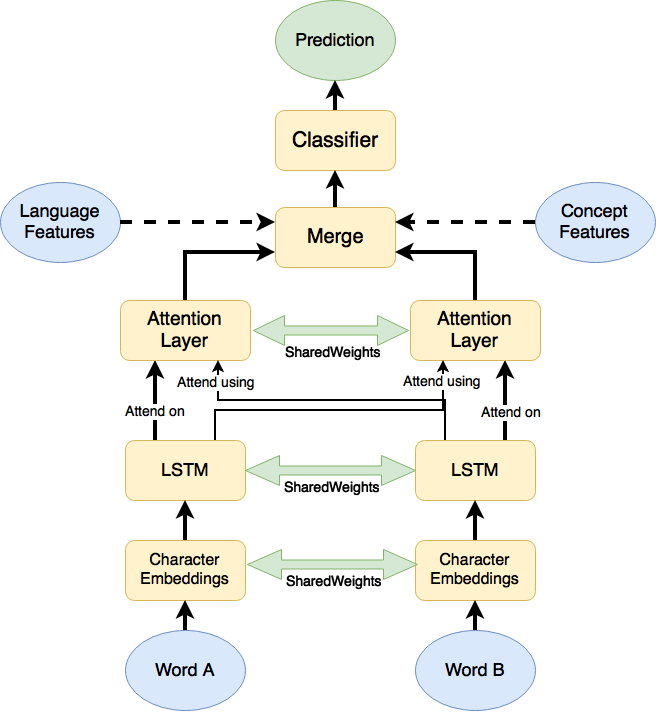
\includegraphics[width=0.7\textwidth]{CoAttNetwork}
    \caption{Recurrent Co-Attention Network for Cognate Discovery}
    \label{CoAttNet}
\end{figure}

The overall model used in our system is called the Recurrent Co-Attention Model (\textit{CoAtt} for short) and is extended from the word-by-word attention model used by Rocktaschel et al.\citep{rocktaschel2016reasoning} for the task of recognising textual entailment in natural language sentences. The network used is illustrated in Figure~\ref{CoAttNet}. It is a Siamese style network that encodes a word pair parallely and then makes a discriminative judgement in the final layer. The input words are first encoded into character level embeddings followed by a bidirectional LSTM network and finally a character by character attention layer as described in the subsections that follow. The encodings of both the words are merged and passed through a 2-layer neural network with \textit{tanh} and \textit{sigmoid} activations to make a final binary prediction. Additionally we also add a \textit{Language features} vector or a \textit{Concept features} vector to the model by concatenating it with the merged attention vector before passing it to the 2-layer neural network.

%%%%%%%%%%%%%%%%%%%%%%
\subsection{Character Embeddings}

The network starts by encoding the input words into their character embeddings. We encode the words using a character level embedding matrix $E \in \mathbb{R}^{n_e \times |C|}$. Here $n_e$ is the size of the character embeddings and $C$ is the vocabulary of all characters. Thus for an input word $x$ which can be represented as sequence of characters $x = \{c_{i_1}, c_{i_2}, ..., c_{i_n}\}$, is transformed into a sequence of vectors $y = \{e_{i_1}, e_{i_2}, ..., e_{i_n}\}$ where $e_j$ is the $j^{th}$ column of the $E$ matrix. This embedding matrix is learnt during training and each column in the matrix represents the embedding vector of the respective token in the vocabulary. 

T.Rama \citep{rama2016siamese} manually defined the character embeddings using various properties of the respective phoneme and fixed these embeddings during training. However, we observe that such a method restricts the power of the distributional representation to world knowledge known to us and letting the embeddings be learnt themselves should help learn a representation that is useful for the task in hand.

%%%%%%%%%%%%%%%%%%%%%%
\subsection{LSTM network}

Recurrent Neural networks (RNN) with Long Short-Term Memory (LSTM) have been extensively been used in several NLP tasks. After the input words to the network are encoded using the character embedding matrix, we transform them use LSTM cells. Given the input words $y = \{e_1, e_2, ..., e_n\}$, at every time step $t$ the LSTM of hidden unit size $n_h$ uses the next input $e_t$, the previous output $h_{t-1}$ and the previous cell state $c_{t-1}$ to compute the next output $h_t$ and the next cell state $c_t$ as follows,

\begin{align}
H &= [e_t h_{t-1}] \\
i_t &= \sigma (W^iH + b^i) \\
o_t &= \sigma (W^oH + b^o) \\
f_t &= \sigma (W^fH + b^f) \\
c_t &= i_t * tanh(W^cH + b^c) + f_t * c_{t-1} \\
h_t &= o_t * tanh(c_t)
\end{align}

Here $W^i$, $W^o$, $W^f$, $W^c \in  \mathbb{R}^{n_e+n_h \times n_h}$ and $b_i$, $b_o$, $b_f$, $b_c \in \mathbb{R}^{n_h}$ are trained weights of the LSTM and $[]$ is the \textit{concatenate} operator. The final output of the LSTM gives us a sequence $\{h_1, h_2, ..., h_n\}$ for every word, where $h_j \in \mathbb{R}^{n_h}$.

The LSTM network essentially helps to give a context aware encoding of the input word. Every output encoding $h_j$ represents an encoding of the $e_j$ character that is aware of its history $\{e_1, e_2, ..., e_{j-1}\}$. It is also popular to use bi-directional LSTMs where the reverse sequence is also fed into the network and then the final outputs are concatenated. Using this mechanism, every output encoding $h_j$ becomes aware of both its past context $\{e_1, e_2, ..., e_{j-1}\}$ and its future context $\{e_{j+1}, e_{j+2}, ..., e_n\}$. We use bi-directional LSTMs in our implementation.

%%%%%%%%%%%%%%%%%%%%%%
\subsection{Attention}

Attention neural networks have been used extensively in tasks like machine translation \citep{mtattention}, image captioning \citep{cpattention} and visual question answering \citep{stackedattention}. The attention mechanism helps to enhance the representation obtained from the LSTM cell state by giving it context that is used for attending. More precisely, we attend over the LSTM encoding of a given word, using a single character encoding of the second word. This helps to generate a weighted representation of the first word, to include its important segments with respect to the second word's character. 

Given a character vector $h \in  \mathbb{R}^{n_h}$ using which we would like to attend on a sequence of character vectors $Y = \{c_1, c_2, ..., c_L\} \in \mathbb{R}^{n_h \times L}$, we generate a set of attention weights $\alpha$ and a attention-weight representation $r \in  \mathbb{R}^{n_h}$ of $Y$ as,

\begin{align}
M &= tanh(W^yY + W^hh*e_L) \\
\alpha &= softmax(w^TM) \\
r &= Y\alpha_t^T
\end{align}

Using the mechanism followed by Rocktaschel et al.\citep{rocktaschel2016reasoning} for word-by-word attention, we employ a character-by-character attention model, wherein we find an attention weighted representation of the first word $Y = \{c_1, c_2, ..., c_L\} \in \mathbb{R}^{n_h \times L}$ at every character of the second word $H = \{h_1, h_2, ..., h_N\} \in \mathbb{R}^{n_h \times N}$.

\begin{align}
M_t &= tanh(W^yY + (W^hh_t + W^rr_{t-1})*e_L) \\
\alpha_t &= softmax(w^TM_t) \\
r_t &= Y\alpha_t^T + tanh(W^tr_{t-1})
\end{align}

Here $W^y$, $W^h$, $W^r$, $W^t \in  \mathbb{R}^{n_h \times n_h}$ and $w \in \mathbb{R}^{n_h}$ are trained weights of the Attention layer. The final output gives us $r_N = r_{YH}$ which can considered as attention weighted representation of $Y$ with respect to $H$. Similarly, we also obtain $r_{HY}$. The final feature vector $r^*$ that is passed to the multi-layer perceptron for classification is the concatenation of these 2 vectors.

\begin{align}
r^* &= [r_{HY} r_{YH}]
\end{align}

 This method of making both the sequences attend over each is called the \textit{Co-Attention} model. At the end of this process of attention, we end up with an embedding representation of each word, that is aware of its own context as well as the context of the other word in the pair.
 
%%%%%%%%%%%%%%%%%%%%%%
\subsection{Language Features}

It is known that some languages are more closely related to each other as compared to other languages. Thus, these languages which are closer would naturally tend to share more cognate pairs than they do with other languages. T. Rama\citep{rama2016siamese} tried to exploit this information about language \textit{relatedness} by providing the network with 2-hot encoding vector that represents the respective languages of the 2 input words being tested. The network would then use this information about the languages to learn which language pairs may be more related using the training data provided.

We follow the same approach and provide the model with these addition \textit{Language Features} before the final classification by the 2-layer MLP. The 2-hot input language pair vector $x_{lang}$ is concatenated with the attention weighted representation of the input words $h^{*}$, before being fed into the final 2-layer perceptron for classification.

%%%%%%%%%%%%%%%%%%%%%%
\subsection{Concept Features}

As the information about the language of the input words can be beneficial for the task of cognate discovery, we hypothesise that information regarding the semantics or the meaning of the input word pair should also be helpful. The word semantics can provide information like the POS category of the word, which can be an useful if some POS classes show higher degree of variation in cognates while others show less.

We implement this by using GloVe word embeddings \citep{pennington2014glove}. Word embeddings are distributional representation of words in a low-dimensional space compared to the vocabulary size and they have been shown to capture semantic information about the words inherently. We use the GloVe embedding for the English concept of the word pair as obtained from the label in the dataset, and input this vector to the network before the final MLP for classification. The word embedding of the concept $x_{concept}$ is concatenated with the attention weighted representation of the input words $h^{*}$, before being fed into the final multi-layer perceptron for classification.

%%%%%%%%%%%%%%%%%%%%%%
\subsection{Cross Family Pre-training}

The three different language families with which we work have completely different origins and are placed across different regions geographically. However, it would be interesting to note if any notion of language evolution is still shared amongst these independently evolved language families. We try to test this hypothesis through the joint learning of the model for these families. To implement this, we instantiate the network with the combined character vocabulary of the two language families. We then train the model till the loss saturates on one language family. This is followed by the training of the model on the second language family, while using the learned weights from the pre-training as the initialization. 


%%%%%%%%%%%%%%%%%%%%%%
\section{Experiments}

We conducted several types of evaluations on our models covering a variety of test for thorough analysis of its performance. In the subsections below we describe the results from these different tests.
The wordlist datasets used in our evaluation can be divided on the basis of languages or concepts for testing and training. We also conducted tests on how cross-family pre-training helps different models and also how the different levels of transcription affects the learning and performance of the models.

%%%%%%%%%%%%%%%%%%%%%%%%
\subsection{Evaluation Metric}

We report the \textit{F-score} and the area under the Precision-Recall curve (\textit{AUC}) as a measure of performance for all our models. \textit{F-score} is computed as the harmonic mean of the \textit{precision} and \textit{recall}\footnote{Precision and Recall is computed on positive labels. Precision = TP/(TP+FP), Recall = TP/(TP+FN)}, when the classifier confidence threshold is 0.5. Since the dataset is heavily biased and contains a majority of negative samples (As can be seen in Tables \ref{CL_count} and \ref{CC_count}), \textit{accuracy} is not a good measure of performance to compare the models.

%%%%%%%%%%%%%%%%%%%%%%%%
\subsection{Cross Language Evaluation}

In the cross language evaluation test, we fixed a random set of 70\% of the languages as the training set of languages and the remaining as the testing set, Then we took words from languages in the training set of languages and all concepts, to form the training samples and similarly for the testing samples. It must be noted that all samples were created by taking words from the same concept .ie. for each word pair in the training and testing set, be it positive or negative, belongs to the same concept.

The training and testing set size details for the different datasets formed using cross language evaluation test can be found in Table 5.1. The results for the cross language evaluation tests are listed in Table 5.2.

%%%%%%%%%%%%%%%%%%%%%%%%
\begin{table*}[t]
\centering
\begin{tabular}{lcccccc}
\multicolumn{1}{c}{\textbf{}} & \multicolumn{2}{c}{\textbf{Indo-European}} & \multicolumn{2}{c}{\textbf{Austronesian}} & \multicolumn{2}{c}{\textbf{Mayan}} \\
\multicolumn{1}{c}{}          & Total               & Positive             & Total               & Positive            & Total           & Positive         \\
Training Samples              & 218,429             & 56,678               & 333,626             & 96,356              & 25,473          & 9,614            \\
Testing Samples               & 9,894               & 2,188                & 20,799              & 5,296               & 1,458           & 441             
\end{tabular}
\caption{Data size for Cross Language Evaluation}
\label{CL_count}
\end{table*}

\begin{table*}[t]
\centering
\begin{tabular}{lcccccc}
\multicolumn{1}{c}{\multirow{2}{*}{\textbf{Model}}} & \multicolumn{2}{c}{\textbf{Indo-European}} & \multicolumn{2}{c}{\textbf{Austronesian}} & \multicolumn{2}{c}{\textbf{Mayan}}                  \\ \cline{2-7} 
\multicolumn{1}{c}{}                                & \textit{F-Score}      & \textit{AUC}       & \textit{F-Score}      & \textit{AUC}      & \textit{F-Score} & \multicolumn{1}{l}{\textit{AUC}} \\ \hline
Gap-weighted Subsequence                            & 59.0                  & 75.5               & 58.8                  & 68.9              & 71.8             & \multicolumn{1}{l}{81.8}         \\ \hline
PhoneticCNN                                         & 73.7                  & 86.1               & 54.6                  & 68.0              & 72.8             & \multicolumn{1}{l}{85.0}         \\
PhoneticCNN + Language Features                     & 62.2                  & 85.4               & 46.8                  & 67.0              & 66.4             & \multicolumn{1}{l}{84.0}         \\
CharacterCNN                                        & 75.3                  & 85.3               & 62.2                  & 71.6              & 75.9             & 85.7                             \\
CharacterCNN + Language Features                    & 70.7                  & 82.6               & 61.4                  & 70.1              & 61.1             & 82.2                             \\ \hline
CoAtt                                               & 83.8                  & 89.2               & 69.0                  & 77.5              & 67.1             & 67.7                             \\
CoAtt + Concept Features                            & \textbf{83.5}         & 90.5               & \textbf{68.9}         & \textbf{77.9}     & 76.2             & 84.2                             \\
CoAtt + Pre-training (Austro)                       & 83.2                  & \textbf{90.6}      & -                     & -                 & \textbf{80.4}    & \textbf{88.3}                    \\
CoAtt + Pre-training (IELex)                        & -                     & -                  & -                     & -                 & 79.6             & 85.2                            
\end{tabular}
\label{CL_res}
\caption{Cross Language Evaluation Results}
\end{table*}
%%%%%%%%%%%%%%%%%%%%%%%%

It is observed that the Recurrent Co-attention model (denoted as \textit{CoAtt}) performs significantly better than the CNN \citep{rama2016siamese} and the Subsequence \citep{rama2015automatic} models for the Indo-European and the Austronesian datasets. For the Mayan dataset, the \textit{CoAtt} model does not learn very well and in fact performs worse than even the subsequence model. This can be due to the small size of the Mayan dataset, which is not sufficient for training the \textit{CoAtt} network. 

Since the mode of evaluation is cross-language, it is intuitive that the additional \textit{Language Features} will not contribute to the performance of the model since the languages of the training and testing set do not overlap and hence the relevant language feature weights for the test set are never learnt. That is, any information about the affinity or interaction between the languages in the training set is not useful for the languages in the testing set, as they are not common. This can clearly be observed in the performance of the CNN models, whos performance deteriorates by a margin with the addition of the \textit{Language features}. Hence, we do not use \textit{Language features} with our model for cross-language evaluation.

On the other hand, the \textit{Concept features} discussed earlier, are found to be useful in improving the performance of the \textit{CoAtt} especially on the Mayan dataset. Using the extra information about the word meaning from the of input pair from the \textit{Concept features}, the \textit{CoAtt} model is able to cross the baseline performance on the Mayan dataset.

The best boost however for the \textit{CoAtt} model on the Mayan dataset comes from pre-training the model on the Austronesian and the Indo-European datasets. Pre-training the model on the other language families gives a good initialisation point to start training for the Mayan dataset. Using this method, the \textit{CoAtt} model is thus able to beat the performance of best CNN model (\textit{CharCNN}) on the Mayan dataset. This also provides evidence to our hypothesis that the \textit{CoAtt} was not able to learn on the Mayan dataset simply because of the lack of enough data to train the network, but pre-training the model on other language families helped to show the true potential of the model on the dataset.

\begin{figure}[ht]
	\centering
	\includegraphics[width=\textwidth]{IELEX_CrossLanguage}
    \caption{PR Curve for Cross Language Evaluation on Indo-European dataset}
    \label{CoAttNet}
\end{figure}

\begin{figure}[ht]
	\centering
	\includegraphics[width=\textwidth]{AUSTRO_CrossLanguage}
    \caption{PR Curve for Cross Language Evaluation on Austro dataset}
    \label{CoAttNet}
\end{figure}

\begin{figure}[ht]
	\centering
	\includegraphics[width=\textwidth]{MAYAN_CrossLanguage}
    \caption{PR Curve for Cross Language Evaluation on Mayan dataset}
    \label{CoAttNet}
\end{figure}

The \textit{CoAtt} model was also tested with the 2 different transcriptions for the IELex dataset, IPA and ASJP. The results for the same are list in Table 5.3. It is observed that the model has almost similar performance in both the transcriptions, however the further analysis (shown later) reveals the different performance over different samples.

\begin{table}[b]
\centering
\label{clett}
\begin{tabular}{lcccc}
\multicolumn{1}{c}{\multirow{2}{*}{\textbf{Model}}} & \multicolumn{2}{c}{\textbf{\begin{tabular}[c]{@{}c@{}}Indo-European\\ (ASJP)\end{tabular}}} & \multicolumn{2}{c}{\textbf{\begin{tabular}[c]{@{}c@{}}Indo-European\\ (IPA)\end{tabular}}} \\ \cline{2-5} 
\multicolumn{1}{c}{}                                & \textit{F-Score}                               & \textit{AUC}                               & \textit{F-Score}                               & \textit{AUC}                              \\ \hline
CoAtt                                               & 83.8                                           & 89.2                                       & 82.2                                           & 89.1                                      \\
CoAtt + Concept Features                            & 83.5                                  & 90.5                              & 82.1                                           & 90.7                                     
\end{tabular}
\caption{Cross Language Evaluation : Transcription Tests}
\end{table}

%%%%%%%%%%%%%%%%%%%%%%%%
\clearpage
\subsection{Cross Concept Evaluation}

The cross concept evaluation, was conducted similar to \citep{rama2016siamese}, wherein the first 70\% of the concepts were taken as training concepts and the remaining concepts as testing. The training and testing pair samples were then created from each set by using words from the same concept. The training and testing set size details formed using cross concept evaluation test can be found in Table 5.4. The results for the cross concept evaluation tests are listed in Table 5.5.

It is observed that the \textit{CoAtt} model gives an almost equal performance for the Indo-European and Austronesian datasets as compared to the CNN models. For Mayan, the \textit{CoAtt} model does not learn very well due to the small size of the data. Even though it is able to beat the Subsequence model in terms of F-score, it is still behind the CNN models by more than 10 points. The cross-concept evaluation test is a more rigorous test for cognate detection as the models have not seen any of the similar word structures during training. Words coming from different concepts would have different sequence structures altogether. Different concepts come from different parts of speech and may contain different levels of variability which is tough for the model to detect if it has not observed it during training.

%%%%%%%%%%%%%%%%%%%%%%%%
\begin{table*}[t]
\centering
\begin{tabular}{lcccccc}
\multicolumn{1}{c}{\textbf{}} & \multicolumn{2}{c}{\textbf{Indo-European}} & \multicolumn{2}{c}{\textbf{Austronesian}} & \multicolumn{2}{c}{\textbf{Mayan}} \\
\multicolumn{1}{c}{}          & Total               & Positive             & Total               & Positive            & Total           & Positive         \\
Training Samples              & 223,666             & 61,856               & 375,693             & 126,081             & 28,222          & 10.482           \\
Testing Samples               & 103,092             & 21,547               & 150,248             & 41,595              & 12,344          & 4,297           
\end{tabular}
\caption{Data size for Cross Concept Evaluation}
\label{CC_count}
\end{table*}

\begin{table*}[t]
\centering
\begin{tabular}{lcccccc}
\multicolumn{1}{c}{\multirow{2}{*}{\textbf{Model}}} & \multicolumn{2}{c}{\textbf{Indo-European}} & \multicolumn{2}{c}{\textbf{Austronesian}} & \multicolumn{2}{c}{\textbf{Mayan}}                   \\ \cline{2-7} 
\multicolumn{1}{c}{}                                & \textit{F-Score}      & \textit{AUC}       & \textit{F-Score}      & \textit{AUC}      & \textit{F-Score} & \multicolumn{1}{l}{\textit{AUC}}  \\ \hline
Gap-weighted Subsequence                            & 51.6                  & 62.0               & 53.1                  & 64.5              & 61.0             & \multicolumn{1}{l}{75.4}          \\ \hline
PhoneticCNN + Language Features                     & \textbf{66.4}         & \textbf{73.2}      & 57.8                  & 66.6              & \textbf{80.6}    & \multicolumn{1}{l}{88.1}          \\
CharacterCNN + Language Features                    & 63.5                  & 70.5               & \textbf{60.9}         & \textbf{70.2}     & 79.6             & \multicolumn{1}{l}{\textbf{89.1}} \\ \hline
CoAtt                                               & 64.8                  & 69.8               & 57.1                  & 61.0              & 70.5             & 74.8                              \\
CoAtt + Language Features                           & 65.6                  & 70.8               & 57.3                  & 62.0              & 69.6             & 71.9                              \\
CoAtt+ Concept Features                             & 64.1                  & 70.6               & 58.0                  & 63.1              & 71.9             & 78.6                              \\
CoAtt + Pre-training (Austro)                       & 65.8                  & 71.0               & \textbf{-}            & \textbf{-}        & 71.1             & 78.4                              \\
CoAtt + Pre-training (IELex)                        & -                     & \textbf{-}         & -                     & -                 & 71.2             & 79.0                             
\end{tabular}
\label{CC_res}
\caption{Cross Concept Evaluation Results}
\end{table*}
%%%%%%%%%%%%%%%%%%%%%%%%
